\documentclass[10pt,a4paper]{article}
\usepackage[margin=2cm]{geometry}
\usepackage{mathptmx}  % Times text and math (Type 1)
\usepackage{graphicx,booktabs,xcolor,float,tabularx,amsmath}
\usepackage[safe]{tipa}
\usepackage{hyperref}
\definecolor{linkblue}{RGB}{0,62,138}
\hypersetup{colorlinks=true,linkcolor=linkblue,citecolor=linkblue,urlcolor=linkblue}
\makeatletter
% section headings: "1. Title" with a normal word space, compact spacing
\renewcommand\@seccntformat[1]{\csname the#1\endcsname.\hspace{0.45em}}
\renewcommand\section{\@startsection{section}{1}{\z@}{-2.4ex \@plus -0.6ex \@minus -0.2ex}{1.0ex \@plus 0.2ex}{\normalfont\large\bfseries}}
\renewcommand\subsection{\@startsection{subsection}{2}{\z@}{-1.9ex \@plus -0.5ex \@minus -0.2ex}{0.7ex \@plus 0.2ex}{\normalfont\normalsize\bfseries}}
% captions: one size everywhere, bold label
\setlength\abovecaptionskip{5pt}\setlength\belowcaptionskip{3pt}
\long\def\@makecaption#1#2{\vskip\abovecaptionskip
  \sbox\@tempboxa{\small\textbf{#1.}\ #2}%
  \ifdim\wd\@tempboxa>\hsize {\small\textbf{#1.}\ #2\par}\else\global\@minipagefalse\hb@xt@\hsize{\hfil\box\@tempboxa\hfil}\fi
  \vskip\belowcaptionskip}
\makeatother
\setlength{\textfloatsep}{10pt plus 2pt minus 2pt}\setlength{\intextsep}{8pt plus 2pt minus 2pt}
\setlength{\parskip}{4pt}\setlength{\parindent}{0pt}
\graphicspath{{../analysis/figures/}}
\newcommand{\code}[1]{\texttt{#1}}

\title{\vspace{-1.2cm}Forced Alignment with the Montreal Forced Aligner\\\large Assignment 2a: pipeline, models, and alignment analysis}
\author{Yash Tyagi\\[2pt]\small Code, TextGrid outputs and setup instructions:\\\footnotesize\url{https://github.com/ashdev-7/iiith-fastspeech2-a2/tree/main/2a_forced_alignment}}
\date{November 2026}

% Hooks used when this report is included in the combined document (combined_report/); empty here.
\providecommand{\partdir}{}
\providecommand{\refshook}{}
% float placement of the 2a figures and tables (the combined document fixes them in place)
\newcommand{\placedfigure}{\figure[tb]}\let\endplacedfigure\endfigure
\newcommand{\placedtable}{\table[tb]}\let\endplacedtable\endtable

\begin{document}
\sloppy
\maketitle
\vspace{-0.6cm}

% Assignment 2a report: content. Compiled by report.tex (standalone) and by combined_report/ (combined).
\section{Setup and data preparation}
\textbf{Tooling.} MFA 3.4.4~\cite{mfa} (Kaldi-based~\cite{kaldi}; conda-forge, run through a portable micromamba environment on Windows 11), Python 3.11.
The whole pipeline is a single re-runnable script (\code{scripts/run\_pipeline.py}): it prepares the corpus, downloads the models, finds OOVs,
builds the dictionaries (G2P), runs \code{mfa validate}, aligns three configurations, adapts and re-aligns, and writes the analysis and figures.

\textbf{Dataset.} 6 utterances, 97.2\,s in total, all 16\,kHz mono 16-bit:
3 long read news paragraphs from the BU Radio News corpus~\cite{buradio} (speaker \textit{f2b}, 25--31\,s, 228 words) and
3 short ISLE~\cite{isle} L2-English learner prompts (\textit{``I said white not bait''}, \textit{``\dots new not no''}, \textit{``\dots bad not bed''}, about 4\,s each).
The corpus was arranged in MFA's layout, with one folder per speaker and a \code{.lab} transcript beside each \code{.wav}.

\textbf{Data preparation} (\code{scripts/prepare\_corpus.py}):
(i) the three \code{F2B*.wav} files are \textbf{NIST SPHERE} files (\code{NIST\_1A} header, uncompressed 16-bit PCM) despite the \code{.wav} extension.
MFA's audio reader (libsndfile) decodes them correctly, so conversion is not strictly required; we rewrite them as standard RIFF/WAVE so that tools trusting the extension read them too.
The samples are untouched: sample counts, rate and the header's recorded min/max match exactly, and every sample is identical (\code{analysis/sanity\_checks.md}), so no timing can change.
(ii) The transcripts needed normalisation so that every token is a lexical word. Each change is logged in \code{corpus/normalization\_log.tsv}:
\code{seventy- six} became \code{seventy six} (numbers broken across lines), the acronyms read letter by letter
\code{S.J.C.'s} became \code{s j c's} and \code{WBUR's} became \code{w b u r's}, \code{de-politicize} became \code{depoliticize}; punctuation was dropped and the text lower-cased.
\code{mfa validate} then reported no unreadable audio, no missing transcripts, no OOVs and no phones without acoustic models.

\section{Dictionaries and acoustic models}
Table~\ref{tab:exps} lists the experiments.
\begin{placedtable}\centering\small
\begin{tabularx}{\linewidth}{@{}p{2.75cm}p{3.7cm}p{5.25cm}X@{}}\toprule
Experiment & Acoustic model & Dictionary & Purpose\\\midrule
\code{arpa\_base} & \code{english\_us\_arpa} 3.0 & \code{english\_us\_arpa} 3.0 + G2P for OOVs & primary system\\
\code{mfa\_ipa} & \code{english\_mfa} 3.1 (IPA) & \code{english\_mfa} 3.1 (MFA default) + \code{english\_us\_mfa} G2P & second acoustic model / phone set\\
\code{mfa\_ipa\_dict\_v300} & \code{english\_mfa} 3.1 (IPA) & \code{english\_mfa} \textbf{3.0} (all variants) + G2P & lexicon as error cause?\\
\code{arpa\_g2p\_custom} & \code{english\_us\_arpa} & \textbf{custom}: all 150 word types G2P-generated, 2-best & dictionary trained from transcripts\\
\code{arpa\_adapted} & \code{english\_us\_arpa} \textbf{MAP-adapted} on this corpus & as \code{arpa\_base} & speaker/channel adaptation\\\bottomrule
\end{tabularx}
\caption[Alignment experiments: acoustic models and dictionaries]{The alignment experiments: acoustic model, pronunciation dictionary and purpose of each.}\label{tab:exps}\end{placedtable}
OOVs (clitic-aware lookup, since MFA splits \textit{'s}) were \textit{dukakis, maffy, melnicove, depoliticize}, plus \textit{judgeships} for \code{english\_mfa}.
G2P is MFA's Pynini-based pair n-gram model~\cite{pynini}; its output is plausible, e.g.\ \textit{dukakis}~\code{D UW0 K AA1 K IH0 S} and \textit{melnicove}~\code{M EH1 L N IH0 K OW2 V}.
The wide beam (\code{--beam 100 --retry\_beam 400}) is there because 25--31\,s utterances are the usual cause of beam failures at the defaults. All 6 files aligned in every experiment. Both pretrained dictionaries are byte-identical (MD5) to the official MFA releases.

\section{Results}
Table~\ref{tab:stats} summarises every experiment, and Fig.~\ref{fig:praat} shows two learner prompts as drawn by Praat; Section~\ref{sec:obs} explains the differences.
\begin{placedtable}\centering\small
\resizebox{\linewidth}{!}{\begin{tabular}{@{}llrrrrrr@{}}\toprule
Experiment & Speaker & Phones & Silence \% & Mean phone (ms) & Phones $\le$30\,ms & Speech log-lik. & Word bound.\ $\Delta$ vs base\\\midrule
arpa\_base & f2b & 1025 & 10.7 & 73.7 & 8.1\% & $-46.99$ & --\\
           & isle & 38 & 59.8 & 132.1 & 0.0\% & $-48.52$ & --\\
mfa\_ipa   & f2b & 993 & 10.8 & 76.1 & 11.9\% & n/c & 14.2\,ms (med.\ 10)\\
           & isle & 37 & \textbf{23.0} & \textbf{260.1} & 0.0\% & n/c & \textbf{167\,ms} (max 2.46\,s)\\
arpa\_g2p\_custom & f2b & 1014 & 10.8 & 74.5 & 9.0\% & $-47.84$ & 4.7\,ms\\
           & isle & 38 & 58.6 & 136.1 & 0.0\% & $-48.35$ & 7.0\,ms\\
arpa\_adapted & f2b & 1025 & 10.7 & 73.8 & 8.0\% & $\mathbf{-46.14}$ & 0.1\,ms\\
           & isle & 38 & 59.8 & 132.1 & 0.0\% & $\mathbf{-47.40}$ & 0.0\,ms\\\bottomrule
\end{tabular}}
\caption[Alignment statistics of all experiments]{Alignment statistics (\code{analysis/summary\_by\_experiment.csv}, \code{agreement\_vs\_arpa\_base.csv}, \code{mfa\_quality\_by\_experiment.csv}).\label{tab:stats}
$\Delta$ = mean absolute difference of word start/end times against \code{arpa\_base}, pooled over all word boundaries. Log-likelihoods (MFA's \code{alignment\_analysis.csv}) are only comparable within the ARPA models (n/c = not comparable).}
\end{placedtable}

\begin{placedfigure}\centering
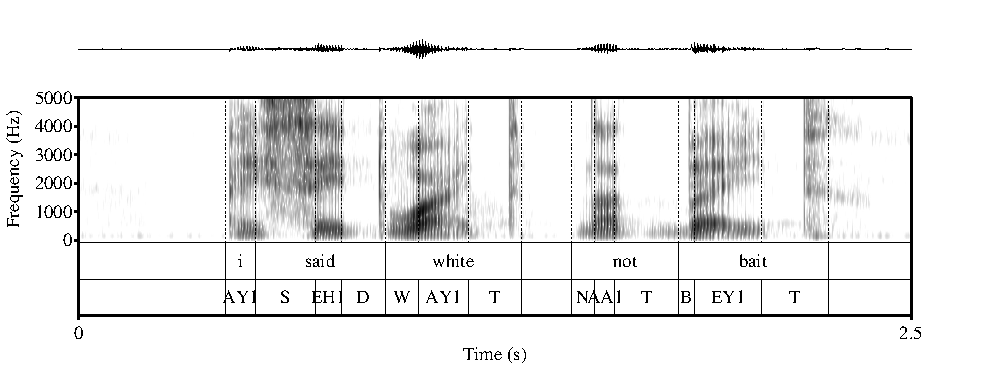
\includegraphics[width=\linewidth]{praat_arpa_base_ISLE_SESS0131_BLOCKD02_01_sprt1.pdf}\\[2pt]
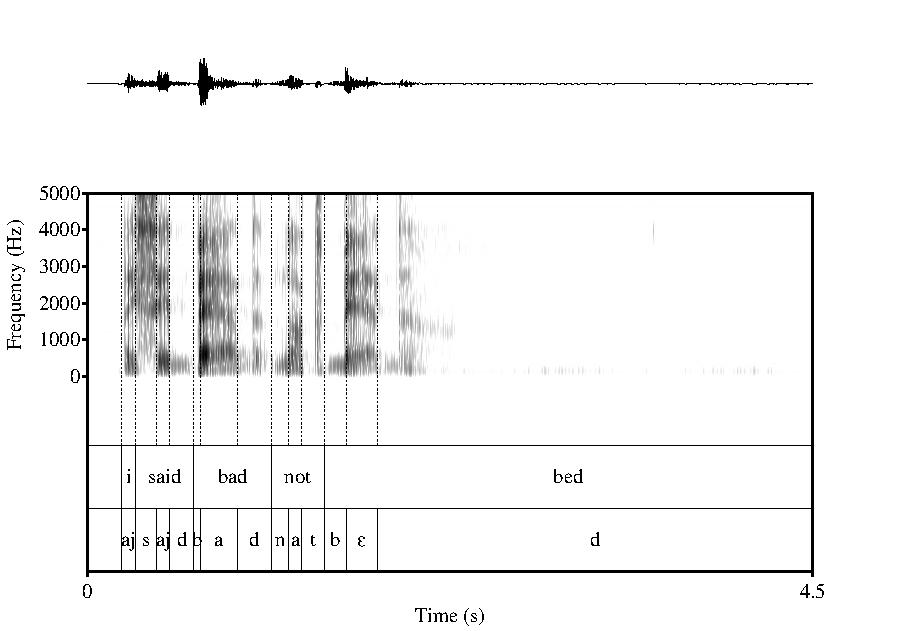
\includegraphics[width=\linewidth]{praat_mfa_ipa_ISLE_SESS0131_BLOCKD02_03_sprt1.pdf}
\caption[Two learner prompts drawn by Praat]{Drawn by \textbf{Praat} 6.1~\cite{praat} (\code{scripts/praat/draw\_alignment.praat}, run headless through parselmouth~\cite{parselmouth} by \code{scripts/praat/run\_praat.py}): waveform, spectrogram, word and phone tiers. Top: \code{arpa\_base} on \textit{``I said white not bait''}. Bottom: \code{mfa\_ipa} on \textit{``I said bad not bed''}, whose final \textit{d} spans 2.5\,s of silence (Error~1). The TextGrids open directly in Praat (\code{View \& Edit}).}\label{fig:praat}
\end{placedfigure}

\section{Observations}\label{sec:obs}
\textbf{How boundaries are placed.} Word boundaries coincide with phone boundaries, because a word interval is exactly the span of its phones, and every boundary sits on MFA's 10\,ms frame grid (all times are multiples of 0.01\,s).
In Fig.~\ref{fig:praat} (top), the pauses between the learner's words are correctly left empty (silence), and each word-final /t/ in \textit{white} and \textit{bait} spans the silent closure plus the visible release burst.
In the read news speech (Fig.~\ref{fig:overlay}), phones are short (median 70\,ms against 120\,ms for the slow, careful L2 speech), and function words get compressed: the five shortest words are all \textit{a} (40--60\,ms).

\textbf{Error 1: the IPA model absorbs pauses into words.} \code{english\_mfa} stretched the last word of two ISLE prompts over the trailing silence:
\textit{bait} runs from 1.70 to 4.13\,s and \textit{bed} from 1.47 to 4.50\,s (Fig.~\ref{fig:praat}, bottom). It also swallowed the 160\,ms pause after \textit{white} and moved the \textit{not}/\textit{bait} boundary 100\,ms early.
On the news speech it absorbed a 250\,ms inter-phrase pause into \textit{he} (Fig.~\ref{fig:overlay}, 7.79--8.04\,s). The three ARPA models put silence in all these places.
This explains its outlier statistics on ISLE: 23\% silence instead of 60\%, a mean phone of 260\,ms, and the largest phone-duration deviation (3.99).
\emph{Praat confirms these stretches are silence} (\code{analysis/praat\_measurements.csv}): the extra 1.88\,s of \textit{bait} and 2.46\,s of \textit{bed} are 24--26\,dB below the speech and 0\% voiced, and the 0.25\,s absorbed into \textit{he} is 12\,dB below and unvoiced.
\emph{It is not the dictionary.} MFA's default \code{english\_mfa} 3.1 dictionary keeps one pronunciation per word, some of them rare variants (\textit{said}~\code{s aj d}, \textit{white}~\code{\textipa{V}aj\textipa{\:t}}).
With the full 3.0 dictionary (\code{mfa\_ipa\_dict\_v300}) the aligner picks \code{s \textipa{E} d} and \code{w aj t}, but absorbs exactly the same silences into \textit{bait} and \textit{bed}. So the lexicon is ruled out, and the evidence points to the acoustic model's silence handling on these short, mostly silent prompts (60\% silence); we did not vary its silence settings, so this mechanism is the most likely one, not a proven one.
Recording noise does not explain it either: by MFA's own estimate the ISLE files are \emph{less} noisy than the news speech (SNR 11.9 vs.\ 8.5\,dB), where the error is rare.
On the news speech, by contrast, the better dictionary does help: 95.2\% instead of 88.2\% of word boundaries within 20\,ms of \code{arpa\_base} (\code{analysis/ipa\_dict\_check.md}).
Not every disagreement is an \code{english\_mfa} error: at \textit{led} (18.16--18.34\,s) the stretch it adds is 67\% voiced and only 1.6\,dB below the speech level, so there the ARPA model may cut the word short.

\textbf{Error 2: very short, near-skipped phones.} 8--12\% of phones in the fast news speech last $\le$30\,ms, the shortest being a single 10\,ms frame.
The most frequent are \code{T} (15), \code{N} (14) and \code{AH0} (8): flapped or unreleased /t/, syllabic or assimilated /n/, and reduced schwas.
The aligner cannot delete a dictionary phone, so a phone the speaker actually elided is squeezed into the minimum duration. These are most likely \emph{skipped phonemes}, although without phone-level hand labels we cannot confirm each one.
The IPA model, with its finer allophone set (e.g.\ separate flap and syllabic phones), produces more of them (11.9\%).

\textbf{Error 3: wrong pronunciations from a G2P-only dictionary.} Without the curated lexicon, the aligner sometimes picks bad G2P variants:
\textit{the} as \code{TH IY0}, \textit{w} as \code{V}, \textit{j} as \code{JH}, \textit{of} as \code{AA1 F}, \textit{these} as \code{TH IY1 Z} (45 differing tokens in \code{pronunciation\_diffs.csv}).
Word boundaries stay close (median 0\,ms, mean 4.8\,ms), but phone labels become wrong and the likelihood on native speech drops (from $-46.99$ to $-47.84$).
For the L2 learner, though, the G2P dictionary fits slightly \emph{better} (from $-48.52$ to $-48.35$), and the aligner chose \textit{said}~\code{S EY1 D} instead of the lexicon's \code{S EH1 D}.
That is a typical spelling pronunciation for L2 speakers, and it shows how pronunciation variants matter for non-native speech.

\textbf{Error 4 (a limitation of forced alignment): it cannot detect mispronunciations.} Alignment is \emph{forced} to the canonical phone sequence.
Whether the learner said \textit{bad} as \code{B AE1 D} or as \code{B EH1 D}, the aligner still labels the vowel \code{AE1}.
Spotting minimal-pair errors would need free phone recognition or goodness-of-pronunciation scoring on top of the alignment.

\textbf{Automatic checks independent of any aligner.} An energy check (\code{energy\_flags.csv}) flags words longer than 0.25\,s whose frames are mostly within 6\,dB of the file's noise floor.
It catches both IPA errors. Its other flags (\textit{court}, \textit{act}, \textit{clerk} in all models) are mostly words that end in a stop closure, a known false-positive type.
An aligner-independent pause reference (\code{scripts/reference\_check.py}) marks every stretch of $\ge$150\,ms within 6, 9 or 12\,dB of the noise floor in Praat's intensity contour.
On ISLE, the ARPA models put $\le$1\% of that pause time inside words at every threshold; \code{english\_mfa} puts 35--56\% there.
This confirms Error~1 without trusting any aligner. The same reference is \emph{too coarse} to rank aligners at the 10--20\,ms level: its edges move with the threshold, and on the news speech it also catches low-energy stretches inside words (stop closures, weak fricatives), equally for every model.

\textbf{Hand-labelled reference} (\code{hand\_labels/}, \code{analysis/hand\_label\_check.md}). The author marked 60 words (120 boundaries: all 15 ISLE words, 45 random news words) by hand, twice, in a tool that shows no aligner output (\code{scripts/marking\_tool.py}; the raw marks of both passes are in \code{hand\_labels/kit/}).
The passes differ by a median of 11\,ms (mean 35\,ms), and pass~2 is 27\,ms later on average. This single-annotator imprecision is as large as the aligners' errors against the mean of the passes (ARPA models: median 22.5--26.3\,ms, 76--77\% within 50\,ms), and the 120 boundaries are not independent (they share words and utterances).
The reference therefore cannot rank the ARPA variants, whose differences are 1--10\,ms, and we draw no statistical conclusion from it. What it does resolve is gross error: \code{english\_mfa} is similar on the news speech, but ends ISLE \textit{bed} and \textit{bait} 2.4 and 1.9\,s late (Error~1), the only gross errors.
The two passes were separate sessions with a night's sleep between them (our protocol had planned a full day), so they may agree slightly more closely than fully independent passes would.

\textbf{Adaptation.} MAP adaptation raises the speech log-likelihood for both speakers (from $-46.99$ to $-46.14$ and from $-48.52$ to $-47.40$) but its boundary changes (99.3\% of word boundaries identical on the news speech and 100\% on ISLE, max 10\,ms) are \emph{indistinguishable from MFA's own run-to-run variation} (below).
With 97\,s of data the Gaussians move only slightly, and the segmentation was already stable.
Note that \code{mfa adapt --output\_directory} exports the \emph{pre}-adaptation alignment (its log says ``Alignment already done, skipping''), so the pipeline re-aligns explicitly with the adapted model.

\begin{placedfigure}\centering
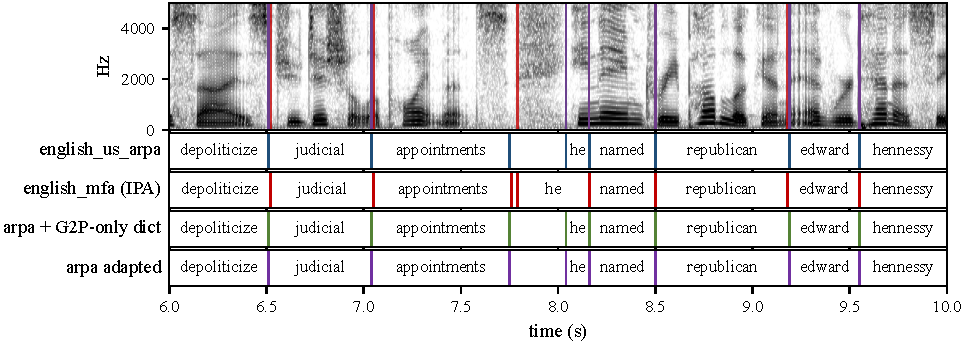
\includegraphics[width=\linewidth]{fig_overlay.pdf}
\caption[Word boundaries of all experiments over one spectrogram]{Word boundaries of all four experiments over one spectrogram (news speech, 6--10\,s of \code{F2BJRLP2}): the ARPA models agree to within 10--20\,ms, and \code{english\_mfa} absorbs the pause before \textit{he}. (The \textit{bed} error is shown by Praat in Fig.~\ref{fig:praat}.)}
\label{fig:overlay}
\end{placedfigure}

\textbf{Sanity checks: does our preparation change the answer, and how repeatable is MFA?} (\code{run\_pipeline.py --stages sanity}, \code{analysis/sanity\_checks.md}).
\emph{Noise floor:} re-running the identical \code{arpa\_base} setup twice leaves 99.3--100\% of word boundaries identical, with differences of at most one 10\,ms frame (phones: $\le$20\,ms). Differences of this size are not meaningful.
\emph{Untouched input:} aligning the provided files exactly as given (SPHERE audio, original transcript text) gives the same word boundaries for every word whose text we did not change (98.4\% identical, max 10\,ms, i.e.\ at the noise floor).
MFA's own text normaliser already handles 4 of our 6 edits (\textit{S.J.C.'s}, \textit{seventy- six}, \dots).
The two that matter: untouched, \textit{WBUR's} and \textit{politicize} are out-of-vocabulary and become a single \code{spn} (spoken-noise) segment with \emph{no phone alignment}; with our edits they get full phone sequences (\code{D AH1 B AH0 L Y UW0 B IY1 Y UW1 AA1 R Z} for the spelled-out call sign), within the same outer word boundaries.
Our preparation therefore only adds phone-level detail for two words; it does not move any other boundary.
By contrast, the G2P-only dictionary changes boundaries well beyond the noise floor (85\% identical, max 250\,ms), so Error~3 is a real effect.

\textbf{Conclusion.} The \code{english\_us\_arpa} acoustic model with its curated dictionary plus G2P for OOVs gives the most reliable alignment of this data.
On the news speech, the second acoustic model agrees with it to a median of 10\,ms (83--88\% of boundaries within 20\,ms), which suggests the boundaries are stable.
The disagreements are concentrated in pause handling on the short L2 prompts, where the spectrogram and energy evidence favour the ARPA model.
The hand-labelled reference confirms the main finding at its resolution: the only gross boundary errors are \code{english\_mfa}'s pause absorptions. It is too coarse to rank the ARPA variants.

\begin{placedfigure}\centering
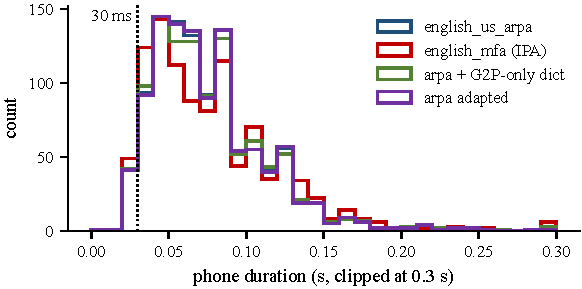
\includegraphics{fig_phone_durations.pdf}
\caption[Phone-duration distributions]{Phone-duration distributions of all experiments (non-silence phones, clipped at 0.3\,s). The mass at $\le$30\,ms is the near-skipped phones of Error~2; the \code{english\_mfa} tail beyond 0.25\,s is its pause-absorption error.}
\label{fig:phonedur}
\end{placedfigure}

\textbf{Deliverables and extra credit.} TextGrids are in \code{outputs/<experiment>/} and figures in \code{analysis/figures/}.
The extra-credit items are a custom G2P-generated dictionary, two pretrained acoustic models plus an adapted one, and a fully automated one-command pipeline. To reproduce everything: \code{conda env create -f environment.yml \&\& conda activate mfa \&\& python scripts/run\_pipeline.py}.
\begin{thebibliography}{9}\footnotesize\setlength\itemsep{0pt}\refshook
\bibitem{mfa} M.~McAuliffe, M.~Socolof, S.~Mihuc, M.~Wagner, and M.~Sonderegger, ``Montreal Forced Aligner: Trainable text-speech alignment using Kaldi,'' in \emph{Proc. Interspeech}, 2017, pp.~498--502.
\bibitem{kaldi} D.~Povey et al., ``The Kaldi speech recognition toolkit,'' in \emph{Proc. IEEE ASRU}, 2011.
\bibitem{pynini} K.~Gorman, ``Pynini: A Python library for weighted finite-state grammar compilation,'' in \emph{Proc. ACL Workshop on Statistical NLP and Weighted Automata}, 2016.
\bibitem{buradio} M.~Ostendorf, P.~J. Price, and S.~Shattuck-Hufnagel, ``The Boston University Radio News Corpus,'' Tech. Rep. ECS-95-001, Boston University, 1995.
\bibitem{isle} W.~Menzel, E.~Atwell, P.~Bonaventura, D.~Herron, P.~Howarth, R.~Morton, and C.~Souter, ``The ISLE corpus of non-native spoken English,'' in \emph{Proc. LREC}, 2000.
\bibitem{praat} P.~Boersma and D.~Weenink, ``Praat: doing phonetics by computer,'' version 6.1, \url{https://www.praat.org}.
\bibitem{parselmouth} Y.~Jadoul, B.~Thompson, and B.~de~Boer, ``Introducing Parselmouth: A Python interface to Praat,'' \emph{Journal of Phonetics}, vol.~71, pp.~1--15, 2018.
\end{thebibliography}


\end{document}
